\chapter{Data}

This chapter describes the background of the data, how it is produced and the expected format.

\section{Source}
The data comes form several medical sensors which are mounted to the bed of the corresponding proband. The sensors send their data in configured intervals to a data pipeline. The pipeline then transforms the data and then saves it in a Postgres DB.

\section{Format}
\label{c:data_format}

The source of the data for this project is stored in a database which implements a star-schema. The data is daily exported to CSV files for each proband using trivial join expressions.

All time series are recorded from 8:00 PM to 10:00 AM.
The sampling granularity is one second. However due to the sensors behaviour, some data points are missing every 30s.
Due to the fine granularity this is negligible.

If data would be sent every second without missing data, each time series would be $14\cdot3600 = 50400$ rows long. However the length is usually around 48000.

\clearpage
The given CSV then contains the following columns:

\begin{multicols}{2}
\begin{itemize}
  \item id
  \item heart\_rate
  \item respiration\_rate
  \item relative\_stroke\_volume
  \item heart\_rate\_variability
  \item measured\_signal\_strength
  \item status
  \item b2b1
  \item b2b2
  \item b2b3
  \item date
  \item day
  \item month
  \item year
  \item location\_name
  \item room
  \item patient
  \item sensor
  \item hour
  \item minute
  \item second
\end{itemize}
\end{multicols}

During the preparation and cleaning process the attributes "date", "hour", "minute" and "second" are used in order to create the timestamps.
For now, the focus will lie on the features "heart\_rate" and "respiration\_rate".


\section{Cleaning}
Due to the fact that real world data is used, some work has to to be put into data cleaning. This work is done in the Jupyter Notebook "CleanAllRawData.ipynb". It is well documented so have a look at it for more information.


The sensor sometimes is not able to detect a signal although the person is in bed. In such case it will send 0-values. Therefore the values of e.g \ac{hr} and \ac{rr} jump quite often to zero.

However even if no heart rate or respiration rate can be detected, the \ac{mss} will produce a high value. Observations have shown, that if the \ac{mss} is below a given threshold (e.g 715) the bed is actually not occupied. In this case the zero-values sent by the sensor are legit. If the \ac{mss} is above the threshold but \ac{hr} and \ac{rr} are zero, this must be considered as missing value.

The forward fill will produce a slight look ahead bias. But due to the fine granularity of the data and the downsampling to come, this is negligible.

We replace these values using a custom forward fill. Figure \ref{fig:forward_fill_example} displays the original time series of \ac{hr} (blue) and the resulting time series after the forward fill algorithm.

\begin{figure}[h!]
	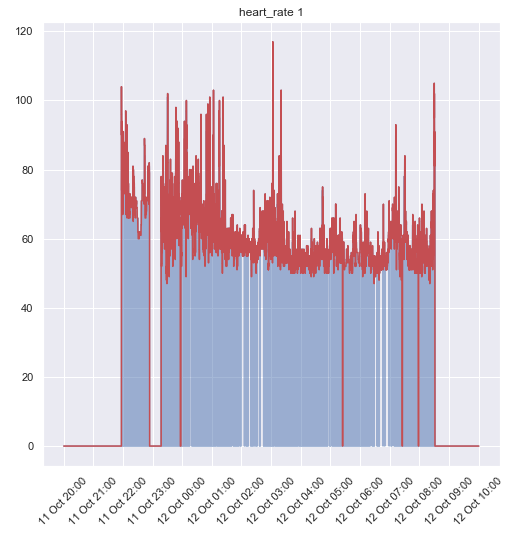
\includegraphics[width=1.1\textwidth]{/forward_fill_example.png}
	\caption{Example of the forward fill output}
	\label{fig:forward_fill_example}
\end{figure}


\newpage
Running time series clustering algorithms is very expensive (regarding computation costs). Therefore the datasets have to been downsampled to different granularities. At the moment the granularities 

\begin{itemize}
	\item 1 hour
	\item 30 minutes
	\item 5 minutes
	\item 1 minute
\end{itemize}

are provided.



\section{Used time series}
After cleaning the raw time series it will be available with the rows \textbf{timestamp}, \textbf{heart rate}, \textbf{respiration rate}, \textbf{mss} and \textbf{patient}. As shown in table \ref{tab:example_ts_one_h_granularity}.


\begin{table}[h!]
\centering
\resizebox{\textwidth}{!}{
	\begin{tabular}{|c|c|c|c|c|}\hline%
		% specify table head
		\bfseries timestamp & 
		\bfseries heart\_rate &
		\bfseries respiration\_rate &
		\bfseries mss &
		\bfseries patient
		
		\csvreader[]{\myCleanedCsvDataPath/samples50/one_hour/yyyyy_1.csv}{
			1=\myTS,2=\myHR,3=\myRR,
			4=\myMSS,5=\myPAT} % specify your columns here
			{\\\hline\myTS & \myHR & \myRR & 
			\myMSS & \myPAT}
		\\\hline	
	\end{tabular}
}
\caption{Example One hour granularity data}
\label{tab:example_ts_one_h_granularity}
\end{table}

For every granularity there are 50 different time series stored in \path{src/data/cleaned/samples/}. Four of them had been synthetically generated using the jupyter notebook \path{synth_data_generator.ipynb}. This was necessary because four data sets had to be discarded during the data cleaning process.
